\documentclass{article} % For LaTeX2e
\usepackage[preprint]{colm2025_conference}

\usepackage{microtype}
\usepackage{hyperref}
\usepackage{url}
\usepackage{booktabs}
\usepackage{graphicx}

\usepackage{lineno}

\definecolor{darkblue}{rgb}{0, 0, 0.5}
\hypersetup{colorlinks=true, citecolor=darkblue, linkcolor=darkblue, urlcolor=darkblue}

\usepackage[most]{tcolorbox}
\tcbuselibrary{listings,breakable}
\usepackage{xcolor}

\definecolor{PromptFrame}{HTML}{4B6584}   % 边框色
\definecolor{PromptBack}{HTML}{F7F9FC}    % 背景色
\definecolor{PromptTitle}{HTML}{1B1F3B}   % 标题文字色

% 适合一小段文本的盒子(不用 verbatim)
\newtcolorbox{promptbox}[2][]{%
  enhanced,
  breakable,
  colback=PromptBack,
  colframe=PromptFrame,
  boxrule=0.4pt,
  arc=1.5mm,
  outer arc=1.5mm,
  fonttitle=\bfseries,
  coltitle=PromptTitle,
  title={#2},
  left=3mm, right=3mm, top=1.5mm, bottom=1.5mm,
  attach boxed title to top left={xshift=2mm,yshift*=-2mm},
  boxed title style={colback=white,arc=1mm,outer arc=1mm},
  #1
}

% 适合直接粘贴完整 prompt(代码风、等宽字体)
\newtcblisting{promptlisting}[2][]{%
  enhanced,
  breakable,
  colback=PromptBack,
  colframe=PromptFrame,
  boxrule=0.4pt,
  arc=1.5mm,
  outer arc=1.5mm,
  fonttitle=\bfseries,
  coltitle=PromptTitle,
  title={#2},
  listing only,
  listing options={
    basicstyle=\ttfamily\small,
    breaklines=true,
    columns=fullflexible,
    keepspaces=true
  },
  left=3mm, right=3mm, top=1.5mm, bottom=1.5mm,
  attach boxed title to top left={xshift=2mm,yshift*=-2mm},
  boxed title style={colback=white,arc=1mm,outer arc=1mm},
  #1
}

\title{Pessimistic Verification for Open Ended Math Questions}

% Authors must not appear in the submitted version. They should be hidden
% as long as the \colmfinalcopy macro remains commented out below.
% Non-anonymous submissions will be rejected without review.

\author{Antiquus S.~Hippocampus, Natalia Cerebro \& Amelie P. Amygdale \thanks{ Use footnote for providing further information
about author (webpage, alternative address)---\emph{not} for acknowledging
funding agencies.  Funding acknowledgements go at the end of the paper.} \\
Department of Computer Science\\
Cranberry-Lemon University\\
Pittsburgh, PA 15213, USA \\
\texttt{\{hippo,brain,jen\}@cs.cranberry-lemon.edu} \\
\And
Ji Q. Ren \& Yevgeny LeNet \\
Department of Computational Neuroscience \\
University of the Witwatersrand \\
Joburg, South Africa \\
\texttt{\{robot,net\}@wits.ac.za} \\
\AND
Coauthor \\
Affiliation \\
Address \\
\texttt{email}
}

% The \author macro works with any number of authors. There are two commands
% used to separate the names and addresses of multiple authors: \And and \AND.
%
% Using \And between authors leaves it to \LaTeX{} to determine where to break
% the lines. Using \AND forces a linebreak at that point. So, if \LaTeX{}
% puts 3 of 4 authors names on the first line, and the last on the second
% line, try using \AND instead of \And before the third author name.

\newcommand{\fix}{\marginpar{FIX}}
\newcommand{\new}{\marginpar{NEW}}

\begin{document}

\ifcolmsubmission
\linenumbers
\fi

\maketitle

\begin{abstract}
  The key limitation of the verification performance lies in the ability of error detection. With this intuition we designed several variants of pessimistic verification, which are simple workflows that could significantly improve the verification of open-ended math questions. In pessimistic verification we conducts multiple reviews on a single proof with a special focus on certain parts, and reports false if any one of them finds an error. This simple technique significantly improves the performance across many math verification benchmarks without introducing too much extra budget. Its token efficiency even surpassed extended long-cot in test-time scaling. Self verification and correction are one of the central perspectives of reasoning and intelligence. This enables an agent to constantly refine its own reasoning or actions, and they are also critical for effectively performing long tasks such as mathematical research. We believe pessimistic verification would be especially useful for many related researches.
\end{abstract}

\section{Introduction}

Since the release of OpenAI o1~\citep{openai_openai_2024} and DeepSeek-R1~\citep{deepseek-ai_deepseek-r1_2025}, reasoning has become one of the most important topics in large language model (LLM) research within both academia and industry. Nevertheless, the scalability of the training recipe behind current large reasoning models (LRMs) is still limited by the requirement of verifiable reward. Even in math, one of the most successful domain of LRM, the absence of a generic verifiable reward still introduces significant challenges to more advanced, open-ended and long-form reasoning tasks~\citep{xu_direct_2025}.

One possible solution to this problem is through formal theorem provers such as Lean~\citep{chen_seed-prover_2025, varambally_hilbert_2025}, which could provide completely reliable verification on math proofs. However, this approach would introduce notable external budget to the AI system and their performance still largely falls behind that of provers in natural language~\citep{dekoninck_open_2025}. Another line of work focuses on leveraging the internal capability of the LLM to achieve self evolution~\citep{zuo_ttrl_2025, yu_rlpr_2025, xu_direct_2025}.

We contend that the importance of self-verification capabilities can be reflected in several key dimensions:

\begin{itemize}
  \item Effective self-verification can substantially enhance the reliability of model outputs and significantly improve overall performance. The performance IMO level math problems can be notably enhanced via a verifier-guided workflow according to \citet{huang_gemini_2025, luong_towards_2025}.
  \item Existing research indicates that the reliability of single-step task execution strongly influences the duration over which a system can operate dependably, thus introspective abilities may be particularly critical for long-horizon tasks~\citep{kwa_measuring_2025}.
  \item We further argue that a general intelligent system should possess intrinsic mechanisms for self-validation, rather than relying exclusively on external ground-truth signals or verification modules.
\end{itemize}

Intuitively we believe that the key limitation of verification lies in the ability of finding errors in a proof, which is also supported by some recent researches~\citep{pandit_hard2verify_2025}. So in this work we introduce three simple workflows which we call \textbf{simple pessimistic verification}, \textbf{vertical pessimistic verification}, and \textbf{progressive pessimistic verification}. These methods imitate the common practice of the review process of math papers, where a paper would be rejected if any one reviewer finds an error in it. They will review a given solution multiple times from different perspectives, and the whole proof will be considered false if any one review finds an error. We have conducted a series of experiments on three datasets, \textit{Hard2Verify}~\citep{pandit_hard2verify_2025}, \textit{IMO-GradingBench}~\citep{luong_towards_2025}, and our homemade \textit{QiuZhen-Bench}. The former two benchmarks are both contest-level math grading benchmarks with expert annotations. \textit{QiuZhenBench} was collected and curated from S.-T. Yau College Student Mathematics Contest and the doctoral qualifying exams fron QiuZhen college, Tsinghua University. These exams covers a wide range of topics in undergraduate-level mathematics and are well-known for their high difficulty. On all benchmarks our methods consistently show impressive improvements in error detection rate and overall f1 score, indicating their effectiveness on proof verifications.

\section{Method}

\begin{figure}[htbp]
  \centering
  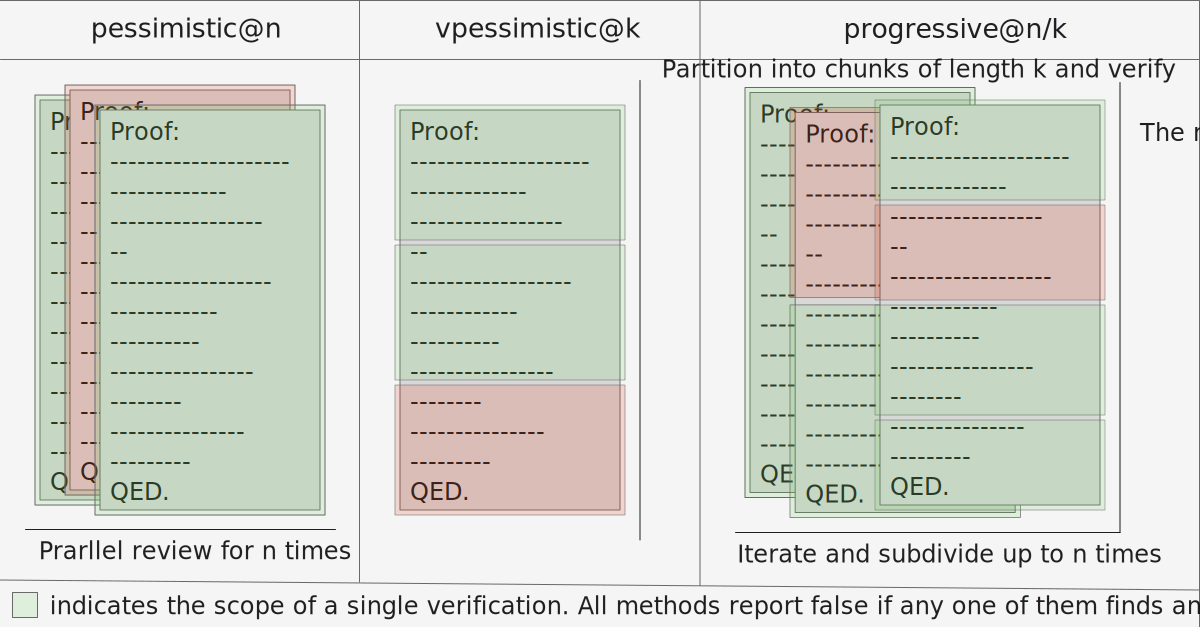
\includegraphics[width=1.0\textwidth]{pessimistic_verifiers.pdf}
  \caption{Three variants of pessimistic verification methods in this work. In following experiments they will separately be denoted as ``pes@n'', ``vp@l'', and ``prog@n/l''}
  \label{fig:pverify-methods}
\end{figure}

\subsection{Metrics}

In this work, we treat mathematical proof verification as a binary classification problem and focus on the following performance metrics:

\begin{itemize}
  \item \textbf{True Negative Rate (TNR)}: The proportion of detected errors among all erroneous proofs. This is the primary metric for evaluating the model’s ability to identify incorrect proofs.
  \item \textbf{True Positive Rate (TPR)}: The proportion of proofs classified as correct among all truly correct proofs. This helps assess the model’s proof-verification capability.
  \item \textbf{Balanced F1 Score}: The harmonic mean of TPR and TNR, providing a balanced indicator of performance when both false positives and false negatives matter. This is also the primary indicator used in \citet{pandit_hard2verify_2025}.
\begin{equation}
  \mathrm{Balanced\ F1} = \frac{2 \cdot \mathrm{TPR} \cdot \mathrm{TNR}}{\mathrm{TPR} + \mathrm{TNR}}
  \label{eq:balanced-f1}
\end{equation}
\end{itemize}

\subsection{Simple pessimistic verification}

A common strategy of enhancing model capability is through majority voting. In majority voting we run the same requests in parallel for multiple times, and choose the majority as final answer. However, this mechanism does not work on verification tasks according to our experiments and some related researches~\citep{pandit_hard2verify_2025}.

In simple pessimistic verification, we conduct multiple reviews on a single proof as majority voting, but instead of using the majority as final answer, we will constantly choose the worst verification from these reviews. As shown in Figure~\ref{fig:pes-vs-maj}, this method drasticly improves the overall performance of evaluation where majority has almost no effect.

We can roughly understand this phenomenon as follows: since the most difficult part of mathematical proof verification is detecting errors, it is likely that only a small number of evaluations can identify the critical mistakes. In this case, majority voting may actually restrict the model’s ability to uncover potential errors, while pessimistic verification further reinforces this ability.

\begin{figure}[htbp]
  \centering
  \includegraphics[width=1.0\textwidth]{./pes_vs_maj.pdf}
  \caption{The comparion of simple pessimistic verification and majority voting. The former exhibits steady performance gains as sampling budget increases, whereas the latter shows almost no changes in performance.}
  \label{fig:pes-vs-maj}
\end{figure}

\subsection{Vertical pessimistic verification}

In spite of simply applying multiple reviews on the whole proof, we also explored a pessimistic verification from another dimension. As shown in Figure~\ref{fig:vertical-prompting}, we adopted a special prompting method and require the LLM to focus on a certain part of the proof, and try looking deep into these contents to find errors. Vertical pessimistic verification adopts a hyperparameter $l$, it first splits the whole proof into chunks with $l$ lines, and create a series of parallel review tasks for each chunk. Although this method only goes through the proof once, we also witnessed improved performance in error detection and even a higher scaling efficiency compared to simple pessimistic verification. 

\begin{figure}[htbp]
  \centering
  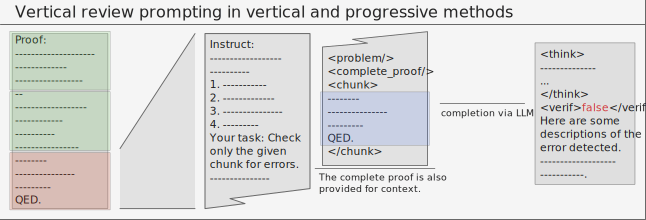
\includegraphics[width=1.0\textwidth]{./vertical_review_prompting.pdf}
  \caption{The vertical review prompting method used in vertical pessimistic verification and progressive pessimistic verification.}
  \label{fig:vertical-prompting}
\end{figure}

\subsection{Progressive pessimistic verification}

Combining the mechanism of both simple and vertical methods we can create a progressive pessimistic verification method. This method starts from the whole proof verification, and then progressively subdivide the proof for up to $n$ times. Each chunk is restricted to contain at least $l$ lines. After this process we can create at most $2^n - 1$ different verification requests on a single proof at different scales. This approach eventually achieved the highest performance under certain sampling budget.

\subsection{Pruning in pessimistic verification}

The mechanism of pessimistic verification also enables pruning in the process. We can implement serial execution at certain levels and stop subsequent checks once an earlier validation detects an error. This allows us to effectively reduce computational resource consumption without sacrificing performance. However, running in a serial manner also slows down execution speed, so we need to find a balance between speed and cost.

The progressive verification approach naturally supports pruning. It can run each round of verification in order from coarse to fine, filtering out incorrect answers step by step. Therefore, in our experiments, pruning is enabled by default for this method, and other approaches can be applied in a similar way. Pruning is especially useful when most of the examples in the dataset are negative examples.

\section{Experiments}

\subsection{Datasets and settings}

In our experiments we primarily use three datasets for evaluation, and we constantly use the same prompt and workflow setting across all these dataset. Here are some descriptions about them:

\begin{itemize}
  \item \textbf{IMO-GradingBench}~\citep{luong_towards_2025}. This dataset contains 1,000 human-graded solutions to IMO-level proof problems from IMO-ProofBench~\citep{luong_towards_2025}, from which we selected a subset with 300 samples for evaluation. This is a challenging test of fine-grained mathematical proof evaluation.
  \item \textbf{Hard2Verify}~\citep{pandit_hard2verify_2025}. Hard2Verify contains 200 challenging problems and solutions from recent math conpetitions such as IMO and Putnam. The solutions are generated by strong models such as GPT-5 and Gemini 2.5 Pro and annotated by humans.
  \item \textbf{QiuZhen-Bench}. This is a homemade collection of advanced math problems, with questions sourced from challenging university-level math competitions. It serves as a supplement to the previous two elementary math competition problem datasets. We randomly selected a subset of 300 problems, had them answered by GPT-5-mini, and used GPT-5 for labeling. This subset can be used to evaluate the performance of weaker models. You can refer to Appendix~\ref{sec:qiuzhen-bench} for more details.
\end{itemize}

All evaluation in our experiments was conducted at the response level, and for IMO-GradingBench, only the responses that obtained fully 7 points are considered correct, otherwise they will all be considered false. And aside from our experiments, we will simply use single pass verification with different reasoning effort setting as the baseline, since we already know that majority voting has almost no effect on evaluation. In all our experiments we set the temperature parameter to 1.0 to ensure the diversity of the response.

\subsection{Performance}

\begin{figure}[htbp]
  \centering
  \includegraphics[width=1.0\textwidth]{tnr_f1_comparison.pdf}
  \caption{The main results on IMO-GradingBench. Thinking mode is enabled for all models if possible, and the reasoning effort of gpt series model is set to medium. This method constantly improves the classification performance across all tested models.}
  \label{fig:main-results}
\end{figure}

\subsection{Scaling potential of pessimistic verification}

\subsection{Case study}

\section{Related work}

Using LLM for evaluation or verification tasks is a natural idea. At the early development stage of LLM, some works have already tried this method on traditional tasks in natural language processing, such as text summarization~\citep{liu_g-eval_2023}, dialog generation~\citep{liu_g-eval_2023}, and machine translation~\citep{zheng_judging_2023}. This approach has achieved some results, but several problems still remain, such as scoring bias~\citep{li_evaluating_2025} and self-inconsistency~\citep{haldar_rating_2025}.

The open-ended math problem lies between the math answering problem and other evaluation problems. It lacks simple and direct means of verification, but its correctness is entirely objective. Existing works in this area primarily focus on the alignment of LLM grading and that of humans. Some of them proposed certain agentic workflows that could enhance this ability~\citep{mahdavi_refgrader_2025, mahdavi_scaling_2025}. Reinforcement learning on manually annotated data also exhibited effectiveness on the evaluation of mathematical proofs~\citep{dekoninck_open_2025}. However, these methods lack the scalability in further enhancing the performance, and they cannot distinguish performance improvements brought by subjective preference alignment from those resulting from objectively discovering new errors. Some work also highlights the importance of error detection, as this is the key ability that separates strong verifiers from weaker ones~\citep{pandit_hard2verify_2025}. Before the release of this work, there is no well-known method that could leverage test-time scaling to obtain better evaluation performance other than scaling long chain of thought~\citep{pandit_hard2verify_2025}.

\section{Conclusion and discussion}

In this work we proposed several variants of pessimistic verification method, which exhibits strong performance and even higher scaling potential than long chain of thought on the evaluation of open-ended math problems. These methods construct multiple different verification queries for a single mathematical proof in different ways, and deems the proof incorrect if any one of these queries determines it to be wrong.

Beyond the existing concrete implementations and results, we believe that the error-centered idea behind pessimistic verification is what truly deserves attention. This approach will naturally make the verification of mathematical problems increasingly stringent, which may also align with the field’s gradual trend toward greater formalization and rigor. It may likewise help guide large language models away from merely computing correct answers and toward generating fully rigorous proofs.

We can also envision several direct applications of pessimistic verification:

\begin{itemize}
  \item Using pessimistic verification in math or code related workflows can further improve the reliability of the response, especially for long-form tasks.
  \item This method can further push the capability frontier of state-of-the-art large models, so there is an opportunity to incorporate it into the training pipeline to further raise the upper limit of large models’ abilities in executing verification and rigorous proof tasks.
\end{itemize}

We are also excited about the future works inspired by our pessimistic verification.

\bibliography{pverify}
\bibliographystyle{colm2025_conference}

\appendix
\section{Appendix}

\subsection{Detail in QiuZhen-Bench}\label{sec:qiuzhen-bench}

QiuZhen-Bench is a dataset covering a wide range of topics in advanced math, including analysis, algebra, machine learning theory, geometry, topology, probability, statistics and theoretical physics. We have collected 143 exam papers from S.-T. Yau College Student Mathematics Contest since 2010, and the doctoral qualifying exams fron QiuZhen college, Tsinghua University since 2023, and required GPT-5 to extract and reformat problems directly from the PDF files. Manual spot checks did not reveal any errors in these extracted contents, indicating the strong capability of GPT-5 in doing this task. We firstly divide the exam papers into pages, and for each page we used the following prompt for extraction:

\begin{promptlisting}{system prompt}
You are a meticulous exam parsing assistant.
Extract ALL distinct problems from the provided text chunks.
Return ONLY valid JSON (no commentary). Focus on problem statements; exclude answers and solutions.
\end{promptlisting}

\begin{promptlisting}{user prompt}
Task: Parse the following exam/contest page images to extract problem statements.
Requirements:
- Identify each separate problem with its number or index if present.
- Preserve math using Markdown and LaTeX (inline `$...$`, display `$$...$$`).
- Do not infer content; only use what appears in the images.
- Only include problems written in English; skip non-English (e.g., Chinese).
- If a problem is mixed-language, include only the English statement; otherwise skip.
- If a problem spans multiple pages in this chunk, include the full statement.
Output strictly as JSON array of objects with keys:
  - problem_number: string (e.g., '1', 'II-3', 'A.1'; use 'unknown' if missing)
  - markdown_statement: string (problem text in Markdown; no solution)
  - section: string|null (e.g., 'Analysis', 'Geometry', or null)
  - tags: array of strings (optional keywords, may be empty)
  - source_pages: array of integers (page numbers within this PDF chunk)
Return ONLY JSON.

fSource: {source.rel_path}\nPages: {chunk.start_page}-{chunk.end_page}
\end{promptlisting}

The problems that spans across two pages is extracted by part and combined in the following processing logic. This results in a dataset containing 1,054 problems in total. Here we provide some samples from this dataset:

\begin{promptbox}{Yau contest 2015, applied math}
Let $G$ be graph of a social network, where for each pair of members there is either no connection, or a positive or a negative one.  An unbalanced cycle in $G$ is a cycle which have odd number of negative edges. Traversing along such a cycle with social rules such as friend of enemy are enemy would result in having a negative relation of one with himself!  A resigning in $G$ at a vertex $v$ of $G$ is to switch the type (positive or negative) of all edges incident to $v$.  Question: Show that one can switch all edge of $G$ into positive edges using a sequence resigning if and only if there is no unbalanced cycle in $G$.
\end{promptbox}

\begin{promptbox}{QiuZhen qualifying 2024 spring, theoretical physics}
$\Pi_{\mu\nu}(q)$ via dimensional regularization (35 points)

At one-loop, the photon propagator in QED receives the correction

$$i\,\Pi_{\mu\nu}(q) = - \int \frac{d^4 p}{(2\pi)^4} \, \mathrm{Tr} \left( i\,\gamma^\nu \, \frac{i}{\not p + \not q - m} \, i\,\gamma^\mu \, \frac{i}{\not p - m} \right),$$

where $\gamma_\mu$ is the gamma matrix and $\not p = p^\mu \gamma_\mu$.

i) 10' Show that this expression can be written as

$$i\,\Pi_{\mu\nu}(q) = -i \int \frac{d^4 p}{(2\pi)^4} \, \frac{N_{\mu\nu}}{D},$$

where

$$N_{\mu\nu} = \operatorname{tr}\,[\gamma_\nu(\not p + \not q + m)\gamma_\mu(\not p - m)]\,, \qquad \frac{1}{D} = \int_0^1 d\alpha \, \frac{1}{D},$$

with

$$D = \big[\,l^2 + \alpha(1-\alpha) q^2 - m^2 + i\epsilon\,\big]^2, \qquad \text{where } l = p + \alpha q.$$

ii) 10' Evaluate $N_{\mu\nu}$ and shift momentum integration from $p$ to $l$ as above.

iii) 10' At the integration step over $l$, perform dimensional regularization by promoting to a $d$-dimensional integral. Derive the expression

$$\Pi_{\mu\nu}(q) = (q_\mu q_\nu - \eta_{\mu\nu} q^2)\,\Pi(q^2),$$

when taking the limit $d \to 4$.

iv) 5' Why does this result ensure gauge invariance?
\end{promptbox}

\begin{promptbox}{Yau contest 2019, analysis individual}
Let $\Omega\subset\mathbb{R}^2$ be a bounded domain with smooth boundary. Prove that, for all $p>1$ and $1\le q<\infty$, for all $f\in L^p(\Omega)$, there exists a unique $u\in H_0^1(\Omega)$, such that $$\Delta u = |u|^{q-1}u + f \quad \text{in } \Omega.$$
\end{promptbox}

\begin{promptbox}{QiuZhen qualifying 2025 fall, algebra}
Suppose $r \le n$ are positive integers. Let $X$ be the subset of $M(n \times n, \mathbb{C})$ consisting of complex $n \times n$ matrices with rank at most $r$. Prove that $X$ is Zariski closed. Find the number of irreducible components of $X$, and calculate the Krull dimension of each irreducible component of $X$.
\end{promptbox}

\subsection{Prompt template}

In our experiments, we use the same evaluation prompt template across all these datasets. For standard, majority voting, and simple pessimistic verification, we use this single-pass verification prompt:

\begin{promptlisting}{system prompt: single pass}
You are an assistant highly proficient in mathematics.
The user will provide a math problem together with its proposed solution, and your task is to verify the correctness of that solution according to the given instruction.
\end{promptlisting}

\begin{promptlisting}{user prompt: single pass}
Here is a math problem and a candidate solution of it, and you need to verify the correctness of this solution. Please check each of the following:

1. The provided content is indeed a math problem and its corresponding solution, rather than unrelated material supplied by mistake.
2. The solution actually derives the conclusion required by the original problem.
3. Every step of calculation and formula derivation in the solution is correct.
4. The hypotheses (conditions) and conclusions of any theorems used are correctly matched and applied.
5. The solution relies only on the conditions given in the problem and does not introduce any additional assumptions to obtain the conclusion.

Consistency and error-severity policy (important):
- If only minor, easily fixable issues exist (e.g., small algebraic slips later corrected, notational typos, superficial formatting), treat the solution as correct overall but briefly note such issues.
- If there is any critical error that undermines correctness (e.g., invalid step, wrong theorem usage without required conditions, uncorrected calculation error leading to a wrong result), treat the solution as incorrect.

Response requirements: If the solution is correct overall (possibly with minor issues), reply with `<verification>true</verification>` and briefly list minor issues if any.
 If the solution is incorrect, reply with `<verification>false</verification>` followed by a concise description of the most harmful error.
 Do not include any restatement of the entire solution or problem.

<problem>{problem}</problem>

<answer>{solution}</answer>
\end{promptlisting}

The first step of progressive pessimistic verifier also adopts the single pass prompt, and for the following verification of subdivisions, we will use the following chunk verification prompt. This prompt is also used in vertical pessimistic verification in our experiments.

\begin{promptlisting}{system prompt: chunk verification}
You are an assistant highly proficient in mathematics.
The user will provide a math problem together with its proposed solution, and your task is to verify the correctness of that solution according to the given instruction.
\end{promptlisting}

\begin{promptlisting}{user prompt: chunk verification}
We provide the original problem and the complete proposed solution for full context. 
Then we provide a specific chunk from the solution for focused checking. 
Your task: Check ONLY the given chunk for errors while considering the overall context.

Checklist:
1. The chunk's reasoning and calculations adhere to mathematical correctness.
2. Any theorems used in the chunk match their hypotheses and conclusions.
3. The chunk does not rely on assumptions not justified by the problem or earlier proven steps.

Consistency and error-severity policy (important):
- If only minor, easily fixable issues exist (e.g., small algebraic slips later corrected, notational typos, superficial formatting), treat the chunk as correct overall but briefly note such issues.
- If there is any critical error that undermines correctness in this chunk (e.g., invalid step, wrong theorem usage without required conditions), treat the chunk as incorrect.

Response requirements: If the chunk is correct overall (possibly with minor issues), reply with `<verification>true</verification>` and briefly list minor issues if any. 
If the chunk is incorrect, reply with `<verification>false</verification>` followed by a concise description of the most harmful error in the proof that you found in the chunk.

f<problem>{problem}</problem>

f<full_answer>{full_proof}</full_answer>

f<chunk_index>{idx}</chunk_index>
f<chunk>{chunk}</chunk>
\end{promptlisting}

\subsection{Original data in experiments}

\subsection{More detailed case studies}\label{sec:case-studies}

In this section we primarily focus on the false negative cases reported by different verifiers, these are the most informative cases in our experiments.

\subsubsection{False negative examples on IMO-GradingBench}

\begin{promptbox}{Case1: problem}
For a positive integer $n$, let $A_{n}$ be the number of perfect powers less than or equal to $n$. Here, a perfect power is a number that can be expressed in the form $a^{b}$, where $a$ is a positive integer and $b$ is an integer greater than or equal to 2. Prove that there are infinitely many $n$ such that $A_{n}$ divides $n+2024$.
\end{promptbox}
\begin{promptbox}{Case1: proof}
Let $S$ be the set of perfect powers. A perfect power is a positive integer that can be expressed in the form $a^b$, where $a$ is a positive integer and $b$ is an integer greater than or equal to 2. The set of perfect powers, sorted in increasing order, is $\{1, 4, 8, 9, 16, 25, 27, \dots\}$.
For a positive integer $n$, $A_n$ is the number of perfect powers less than or equal to $n$. So, $A_n = |S \cap \{1, 2, \dots, n\}|$.
The function $A_n$ is a non-decreasing step function. It is constant between consecutive perfect powers. Let $p_k$ denote the $k$-th perfect power. For any integer $n$ in the range $p_k \le n < p_{k+1}$, the value of $A_n$ is constant and equal to $k$.

We want to prove that there are infinitely many positive integers $n$ such that $A_n$ divides $n+2024$.

Our strategy is to find an infinite sequence of disjoint integer intervals, and in each interval, find one such integer $n$.
Let's consider an interval $[p_k, p_{k+1}-1]$ where $A_n$ is constant, equal to $k$. The condition we want to satisfy is $k \mid (n+2024)$. This is equivalent to the congruence relation $n \equiv -2024 \pmod{k}$.
The interval $[p_k, p_{k+1}-1]$ contains $p_{k+1}-p_k$ consecutive integers. If the length of this interval is at least $k$, the integers it contains form a complete residue system modulo $k$. In such a case, there is guaranteed to be an integer $n$ in the interval satisfying $n \equiv -2024 \pmod{k}$.

So, the problem reduces to showing that there are infinitely many values of $k$ for which the gap between consecutive perfect powers, $p_{k+1}-p_k$, is greater than or equal to $k$.

We will focus on a special subsequence of perfect powers: the squares. Consider the gaps between consecutive squares. Let $m \ge 2$ be an integer. We will analyze the interval of integers $I_m = [(m-1)^2, m^2-1]$. We will show that for all sufficiently large $m$:
1.  $A_n$ is constant for all $n \in I_m$. To do this, we will prove that there are no perfect powers in the open interval $((m-1)^2, m^2)$.
2.  The length of the interval $I_m$ is greater than the value of $A_n$ for $n \in I_m$.

If these two conditions hold for some large $m$, let $k_m$ be the constant value of $A_n$ on $I_m$. The length of $I_m$ is $(m^2-1) - (m-1)^2 + 1 = 2m-1$. Condition 2 means $2m-1 > k_m$. As argued above, since the interval $I_m$ contains $2m-1 > k_m$ consecutive integers, there must exist an integer $n_m \in I_m$ such that $n_m \equiv -2024 \pmod{k_m}$. For this $n_m$, we have $A_{n_m}=k_m$, and thus $A_{n_m} \mid (n_m+2024)$.

If we can show that these conditions hold for all $m$ greater than some integer $M$, we can find a solution $n_m$ for each $m \ge M$. Since the intervals $I_m$ are disjoint for different $m$, the solutions $n_m$ will be distinct, proving that there are infinitely many such integers.

We now formalize and prove these two main claims.

**Claim 1:** For all sufficiently large integers $m$, there are no perfect powers in the open interval $((m-1)^2, m^2)$.

**Proof:**
A perfect power in the interval $((m-1)^2, m^2)$ cannot be a perfect square, as there are no integers between $m-1$ and $m$. Therefore, any such perfect power must be of the form $x^j$ where $x \ge 2$ and $j \ge 3$ are integers.
For $x^j$ to be in the interval, we must have $(m-1)^2 < x^j < m^2$.
Taking the $j$-th root of this inequality gives $(m-1)^{2/j} < x < m^{2/j}$.
For an integer $x$ to exist in this range, the length of the interval $((m-1)^{2/j}, m^{2/j})$ must be greater than 1 for some $j$.
The possible values for the exponent $j$ are limited by the condition $2^j \le x^j < m^2$, which implies $j < 2\log_2 m$.

Let $N(a, b)$ be the number of perfect powers in the open interval $(a, b)$. The total number of perfect powers in $((m-1)^2, m^2)$ is bounded by the sum of the number of integer candidates for the base $x$ over all possible prime exponents $j$. For simplicity, we sum over all integers $j \ge 3$:
$$N((m-1)^2, m^2) \le \sum_{j=3}^{\lfloor 2\log_2 m \rfloor} \left( \lfloor m^{2/j} \rfloor - \lceil (m-1)^{2/j} \rceil + 1 \right)$$
A simpler bound is the sum of the lengths of the intervals for $x$:
$$N((m-1)^2, m^2) \le \sum_{j=3}^{\lfloor 2\log_2 m \rfloor} \left( m^{2/j} - (m-1)^{2/j} \right)$$
Let's analyze the term $m^{2/j} - (m-1)^{2/j}$. By the Mean Value Theorem applied to the function $f(t) = t^{2/j}$ on the interval $[m-1, m]$, for each $j$ there exists some $c_j \in (m-1, m)$ such that:
$$m^{2/j} - (m-1)^{2/j} = f'(c_j) \cdot (m - (m-1)) = \frac{2}{j}c_j^{\frac{2}{j}-1}$$
Since $j \ge 3$, the exponent $\frac{2}{j}-1$ is negative. As $c_j > m-1$, we have $c_j^{\frac{2}{j}-1} < (m-1)^{\frac{2}{j}-1}$.
So, $m^{2/j} - (m-1)^{2/j} < \frac{2}{j}(m-1)^{\frac{2}{j}-1}$.

Now we bound the sum. For $j \ge 3$, the exponent $\frac{2}{j}-1 \le \frac{2}{3}-1 = -\frac{1}{3}$.
Assuming $m-1 \ge 1$, we have $(m-1)^{\frac{2}{j}-1} \le (m-1)^{-1/3}$.
$$N((m-1)^2, m^2) < \sum_{j=3}^{\lfloor 2\log_2 m \rfloor} \frac{2}{j}(m-1)^{\frac{2}{j}-1} \le \sum_{j=3}^{\lfloor 2\log_2 m \rfloor} \frac{2}{3}(m-1)^{-1/3}$$
The number of terms in the summation is $\lfloor 2\log_2 m \rfloor - 2 < 2\log_2 m$.
$$N((m-1)^2, m^2) < (2\log_2 m) \cdot \frac{2}{3}(m-1)^{-1/3} = \frac{4 \log_2 m}{3(m-1)^{1/3}}$$
As $m \to \infty$, this upper bound tends to 0. To see this formally:
$$ \lim_{m\to\infty} \frac{4 \log_2 m}{3(m-1)^{1/3}} = \lim_{m\to\infty} \frac{4 \ln m}{3 \ln 2 \cdot (m-1)^{1/3}} = 0 $$
since any positive power of $m$ grows faster than any power of $\ln m$.
Since $N((m-1)^2, m^2)$ must be a non-negative integer, there must exist an integer $M_1$ such that for all $m \ge M_1$, $N((m-1)^2, m^2) = 0$. This proves Claim 1.

**Claim 2:** For all sufficiently large integers $m$, $2m-1 > A_{(m-1)^2}$.

**Proof:**
We need an upper bound for $A_n$. The set of perfect powers is the union of the sets of squares, cubes, 5th powers, and so on. A simple upper bound for $A_n$ is obtained by summing the number of $j$-th powers up to $n$ for all $j \ge 2$, ignoring overlaps which leads to overcounting.
The number of $j$-th powers up to $n$ is $\lfloor n^{1/j} \rfloor$.
$$ A_n \le \sum_{j=2}^{\lfloor \log_2 n \rfloor} \lfloor n^{1/j} \rfloor < \sum_{j=2}^{\lfloor \log_2 n \rfloor} n^{1/j} $$
We can write this as:
$$ A_n < n^{1/2} + n^{1/3} + n^{1/4} + \dots + n^{1/\lfloor\log_2 n\rfloor} $$
The number of terms in the sum after $n^{1/2}$ is $\lfloor \log_2 n \rfloor - 2$. For $j \ge 3$, we have $n^{1/j} \le n^{1/3}$ (for $n \ge 1$).
So, we can bound the sum as:
$$ A_n < n^{1/2} + (\lfloor \log_2 n \rfloor - 2)n^{1/3} < n^{1/2} + (\log_2 n) n^{1/3} $$
Now, let's apply this bound to $A_{(m-1)^2}$. Let $n = (m-1)^2$.
$$ A_{(m-1)^2} < \sqrt{(m-1)^2} + (\log_2((m-1)^2)) \cdot ((m-1)^2)^{1/3} $$
$$ A_{(m-1)^2} < m-1 + (2\log_2(m-1)) \cdot (m-1)^{2/3} $$
We want to prove that $2m-1 > A_{(m-1)^2}$ for sufficiently large $m$. It is sufficient to show that:
$$ 2m-1 > m-1 + 2\log_2(m-1) \cdot (m-1)^{2/3} $$
This inequality simplifies to:
$$ m > 2\log_2(m-1) \cdot (m-1)^{2/3} $$
For $m > 1$, we can divide by $m^{2/3}$:
$$ m^{1/3} > 2\log_2(m-1) \cdot \left(\frac{m-1}{m}\right)^{2/3} = 2\log_2(m-1) \cdot \left(1 - \frac{1}{m}\right)^{2/3} $$
As $m \to \infty$, the term $(1-1/m)^{2/3}$ approaches 1. The inequality will hold if $m^{1/3}$ grows faster than $2\log_2(m-1)$. To confirm this, we examine the limit of their ratio:
$$ \lim_{x\to\infty} \frac{x^{1/3}}{2\log_2(x-1)} = \lim_{x\to\infty} \frac{x^{1/3} \ln 2}{2 \ln(x-1)} $$
Using L'Hôpital's rule on this $\frac{\infty}{\infty}$ form:
$$ = \lim_{x\to\infty} \frac{\frac{1}{3}x^{-2/3} \ln 2}{2 \cdot \frac{1}{x-1}} = \lim_{x\to\infty} \frac{\ln 2}{6} \frac{x-1}{x^{2/3}} = \lim_{x\to\infty} \frac{\ln 2}{6} (x^{1/3} - x^{-2/3}) = \infty $$
Since this limit is infinite, $x^{1/3}$ grows faster than any constant multiple of $\log_2(x-1)$.
Therefore, there exists an integer $M_2$ such that for all $m \ge M_2$, the inequality $m^{1/3} > 2\log_2(m-1) \cdot (1 - 1/m)^{2/3}$ holds. This proves Claim 2.

**Conclusion**

Let $M = \max(M_1, M_2)$. For every integer $m \ge M$, we have established the following:
1.  From Claim 1, the interval $((m-1)^2, m^2)$ contains no perfect powers. This means that for any integer $n$ in the interval $I_m = [(m-1)^2, m^2-1]$, the set of perfect powers less than or equal to $n$ is the same as the set of perfect powers less than or equal to $(m-1)^2$.
    Thus, $A_n$ has a constant value for all $n \in I_m$. Let this value be $k_m = A_{(m-1)^2}$.

2.  From Claim 2, the inequality $2m-1 > A_{(m-1)^2} = k_m$ holds.
    The length of the interval $I_m$ is $(m^2-1) - (m-1)^2 + 1 = 2m-1$.
    So, for $m \ge M$, the length of the interval $I_m$ is strictly greater than $k_m$.

We are looking for an integer $n$ such that $A_n \mid (n+2024)$. For any $m \ge M$, we seek an $n \in I_m$ satisfying $k_m \mid (n+2024)$. This is equivalent to finding an $n$ in the range $(m-1)^2 \le n \le m^2-1$ that satisfies the congruence:
$$n \equiv -2024 \pmod{k_m}$$
The interval $I_m$ contains the sequence of consecutive integers $(m-1)^2, (m-1)^2+1, \dots, m^2-1$. The length of this sequence is $2m-1$. Since $m \ge M$, we have $2m-1 > k_m$. Because the sequence of integers in $I_m$ is longer than a full cycle of residues modulo $k_m$, it is guaranteed to contain at least one integer from each residue class modulo $k_m$.
In particular, there must exist an integer $n_m \in I_m$ such that $n_m \equiv -2024 \pmod{k_m}$.
For this $n_m$, we have $A_{n_m} = k_m$, and so $A_{n_m} \mid (n_m+2024)$.

For each integer $m \ge M$, we have successfully found an integer $n_m$ that satisfies the given property. To complete the proof, we must show that this process generates an infinite number of distinct solutions.

Let $m$ and $m'$ be two integers such that $M \le m < m'$.
The solution $n_m$ lies in the interval $I_m = [(m-1)^2, m^2-1]$.
The solution $n_{m'}$ lies in the interval $I_{m'} = [(m'-1)^2, (m')^2-1]$.
Since $m' > m$, we must have $m' \ge m+1$.
The smallest value in the interval $I_{m'}$ is $(m'-1)^2 \ge (m+1-1)^2 = m^2$.
The largest value in the interval $I_m$ is $m^2-1$.
So, for any $n \in I_m$ and $n' \in I_{m'}$, we have $n \le m^2-1 < m^2 \le n'$. This shows that the intervals $I_m$ and $I_{m'}$ are disjoint.
Consequently, the solutions $n_m \in I_m$ and $n_{m'} \in I_{m'}$ are distinct.

Since we can choose any integer $m \ge M$, we have constructed an infinite sequence of distinct solutions $\{n_m\}_{m \ge M}$.
Therefore, there are infinitely many integers $n$ such that $A_n$ divides $n+2024$.
\end{promptbox}

The manually annotated label in the dataset is true (7 points), while our method found a critical error in it:

\begin{promptbox}{Case1: review from GPT-5-mini}
<verification>false</verification>

The main (fatal) error is in Claim~1: the author replaces the integer count
\[
\bigl\lfloor m^{2/j} \bigr\rfloor - \bigl\lceil (m-1)^{2/j} \bigr\rceil + 1
\]
by the real length \(m^{2/j} - (m-1)^{2/j}\). That inequality is not valid in general
(e.g.\ an interval of real length \(<1\) can still contain an integer). Thus the bound
\[
N\bigl((m-1)^2,m^2\bigr) \le \sum_j \bigl(m^{2/j} - (m-1)^{2/j}\bigr)
\]
is unjustified, and the conclusion “this sum \(\to 0 \Rightarrow N = 0\) for large \(m\)”
does not follow. Because of this mistake the proof does not establish that the open
interval \(\bigl((m-1)^2,m^2\bigr)\) contains no perfect powers for all large \(m\), and
the rest of the argument (which depends critically on that claim) fails.
\end{promptbox}
\begin{promptbox}{Case1: our comment}
The gt\_label is wrong, the pred\_label is correct.

Fatal error in Claim 1: It is invalid to use the length of a real interval to upper-bound the number of integer points, because when the interval length is < 1 it may still contain integers. Therefore, the conclusion ``limit = 0 => final result = 0'' does not hold; Moreover, the proof has a totally wrong derivation that

$$N((m-1)^2, m^2) \le \sum_{j=3}^{\lfloor 2\log_2 m \rfloor} \left( \lfloor m^{2/j} \rfloor - \lceil (m-1)^{2/j} \rceil + 1 \right)$$
$$\Rightarrow N((m-1)^2, m^2) \le \sum_{j=3}^{\lfloor 2\log_2 m \rfloor} \left( m^{2/j} - (m-1)^{2/j} \right)$$

which is actually an unacceptable gap.
\end{promptbox}

\begin{promptbox}{Case2: problem}
  Prove that there exist two real-coefficient polynomials $P(x)$ and $Q(x)$ satisfying the following condition:
  
  (Condition) The degree of the polynomial $P(x)$ is at least 2024, the degree of $Q(x)$ is at least 2, and for any real number $x$, the following holds:
  \[ P(Q(x)-x-1)=Q(P(x))\]
\end{promptbox}

\begin{promptbox}{Case2: proof}
  We will prove the existence of such polynomials $P(x)$ and $Q(x)$ by constructing them. Our construction will follow three main steps:
1. Find a pair of polynomials of low degree, let's call them $(P_0(x), Q_0(x))$, that satisfies the given functional equation.
2. Construct a high-degree polynomial, let's call it $R(x)$, that commutes with $Q_0(x)$.
3. Combine these polynomials to form the final pair $(P(x), Q(x))$ that satisfies all the given conditions.

Let the given equation be
\[P(Q(x)-x-1) = Q(P(x)) \quad (*).\]

\textbf{Step 1: Finding a base solution pair}

We look for a simple solution where $P_0(x)$ and $Q_0(x)$ have degree 2. Let's try to relate them. A simple assumption is that $Q_0(x)$ is a linear perturbation of $P_0(x)$. Let's try the ansatz:
\[Q_0(x) = P_0(x) + x + c\]
for some real constant $c$.
Substituting this into the equation $(*)$:
The left side's argument becomes $Q_0(x)-x-1 = (P_0(x)+x+c) - x - 1 = P_0(x)+c-1$.
So the equation becomes $P_0(P_0(x)+c-1) = Q_0(P_0(x))$.

Let $y = P_0(x)$. For any value $y$ in the range of $P_0(x)$, the equation must hold:
\[P_0(y+c-1) = Q_0(y).\]
Using our ansatz for $Q_0(y)$, we have $Q_0(y) = P_0(y) + y + c$.
So, we obtain a functional equation for $P_0(y)$:
\[P_0(y+c-1) = P_0(y) + y + c.\]
Let $b = c-1$, so $c = b+1$. The equation is
\[P_0(y+b) - P_0(y) = y+b+1.\]
Let $m = \deg(P_0)$. If $b \neq 0$, the degree of the polynomial on the left, $P_0(y+b) - P_0(y)$, is $m-1$. The degree of the polynomial on the right is 1.
For the identity to hold, the degrees must be equal, so $m-1 = 1$, which implies $m=2$.

Let $P_0(y) = Ay^2+By+C$ for some constants $A, B, C \in \mathbb{R}$ with $A \
eq 0$.
Substituting this into the difference equation:
$A(y+b)^2+B(y+b)+C - (Ay^2+By+C) = y+b+1$
$A(y^2+2by+b^2)+B(y+b)+C - =Ay^2-By-C = y+b+1$
$2Aby + Ab^2+Bb = y+b+1$.
This must be a polynomial identity in $y$. We can equate the coefficients of the powers of $y$:
1. Coefficient of $y$: $2Ab = 1$.
2. Constant term: $Ab^2+Bb = b+1$.

This is a system of two equations with three unknowns ($A, B, b$). We can choose a value for one of them. Let's choose $b=2$.
From (1): $2A(2) = 1 \implies 4A=1 \implies A=1/4$.
Substitute $A=1/4$ and $b=2$ into (2):
$(1/4)(2^2) + B(2) = 2+1 \implies 1+2B = 3 \implies 2B=2 \implies B=1$.
The constant $C$ can be any real number. For simplicity, we choose $C=0$.
So, we have found a polynomial $P_0(x) = \frac{1}{4}x^2+x$.
We have $b=2$, so $c=b+1=3$.
Now we find the corresponding $Q_0(x)$:
$Q_0(x) = P_0(x)+x+c = (\frac{1}{4}x^2+x) + x + 3 = \frac{1}{4}x^2+2x+3$.

So, we have found a base solution pair:
$P_0(x) = \frac{1}{4}x^2+x$
$Q_0(x) = \frac{1}{4}x^2+2x+3$
Both have degree 2, satisfying the degree condition for $Q_0(x)$. Let's verify that they satisfy $(*)$.
$Q_0(x)-x-1 = (\frac{1}{4}x^2+2x+3)-x-1 = \frac{1}{4}x^2+x+2$.
LHS: $P_0(Q_0(x)-x-1) = P_0(\frac{1}{4}x^2+x+2) = \frac{1}{4}(\frac{1}{4}x^2+x+2)^2 + (\frac{1}{4}x^2+x+2) = \frac{1}{64}x^4+\frac{1}{8}x^3+\frac{3}{4}x^2+2x+3$.
RHS: $Q_0(P_0(x)) = \frac{1}{4}(P_0(x))^2+2P_0(x)+3 = \frac{1}{4}(\frac{1}{4}x^2+x)^2 + 2(\frac{1}{4}x^2+x)+3 = \frac{1}{64}x^4+\frac{1}{8}x^3+\frac{3}{4}x^2+2x+3$.
LHS=RHS, so the pair $(P_0, Q_0)$ is a solution.

\textbf{Step 2: Construction of a high-degree commuting polynomial}

Our plan is to set $Q(x) = Q_0(x)$ and $P(x) = R(P_0(x))$ for some polynomial $R(x)$ with high degree. Let's see what condition $R(x)$ must satisfy.
Substitute $P(x)=R(P_0(x))$ and $Q(x)=Q_0(x)$ into $(*)$:
LHS: $P(Q(x)-x-1) = R(P_0(Q_0(x)-x-1))$.
Using the property of our base solution, $P_0(Q_0(x)-x-1)=Q_0(P_0(x))$, we get:
LHS = $R(Q_0(P_0(x)))$.
RHS: $Q(P(x)) = Q_0(R(P_0(x)))$.
So, the equation becomes $R(Q_0(P_0(x))) = Q_0(R(P_0(x)))$.
Let $y=P_0(x)$. This identity must hold for all values $y$ in the range of $P_0$. If we find a polynomial $R$ that commutes with $Q_0$, i.e., $R(Q_0(y)) = Q_0(R(y))$ for all $y$, then our equation will be satisfied. Since this is a polynomial identity, if it holds for all $y$ in the range of $P_0$ (an infinite set), it holds for all $y$.

We need to find a polynomial $R(x)$ that commutes with $Q_0(x)$. A standard method for finding commuting polynomials is to simplify $Q_0(x)$ by a linear change of variables (conjugation).
$Q_0(x) = \frac{1}{4}x^2+2x+3 = \frac{1}{4}(x^2+8x) + 3 = \frac{1}{4}(x^2+8x+16) - 4+3 = \frac{1}{4}(x+4)^2 - 1$.
Let $L(x) = x+4$. Its inverse is $L^{-1}(x) = x-4$.
Let $S(y) = \frac{1}{4}y^2-1$.
Then $Q_0(x) = L^{-1}(S(L(x)))$.

If we find a polynomial $\tilde{R}(y)$ that commutes with $S(y)$, then $R(x) = L^{-1}(\tilde{R}(L(x)))$ will commute with $Q_0(x)$. This is because:
$R(Q_0(x)) = L^{-1}(\tilde{R}(L(L^{-1}(S(L(x)))))) = L^{-1}(\tilde{R}(S(L(x))))$.
$Q_0(R(x)) = L^{-1}(S(L(L^{-1}(\tilde{R}(L(x)))))) = L^{-1}(S(\tilde{R}(L(x))))$.
Since $\tilde{R}$ and $S$ commute, $\tilde{R}(S(y))=S(\tilde{R}(y))$, so $R$ and $Q_0$ commute.

A simple way to find a polynomial that commutes with $S(y)$ is to take iterates of $S(y)$. Let $S_1(y) = S(y)$ and $S_k(y) = S(S_{k-1}(y))$ for $k \ge 2$. Then $S_k(y)$ commutes with $S(y)$ for any $k \ge 1$.
Let's choose $\tilde{R}(y) = S_k(y)$ for a sufficiently large $k$.
The degree of $S(y)$ is 2. The degree of $\tilde{R}(y)=S_k(y)$ is $2^k$.
We define $R(x) = L^{-1}(S_k(L(x))) = S_k(x+4)-4$. The degree of $R(x)$ is $2^k$.

\textbf{Step 3: Assembling the final solution}

We are now ready to define $P(x)$ and $Q(x)$.
- Let $Q(x) = Q_0(x) = \frac{1}{4}x^2+2x+3$.
- Let $R(x)$ be constructed with $k=10$, so $\tilde{R}(y) = S_{10}(y) = S^{\circ 10}(y)$, and $R(x) = S_{10}(x+4)-4$.
- Let $P(x) = R(P_0(x)) = R(\frac{1}{4}x^2+x)$.

Let's check the conditions:
1. **Coefficients**: $P_0, Q_0, L, L^{-1}, S$ are all real-coefficient polynomials. Any composition or iteration will also result in polynomials with real coefficients. So $P(x)$ and $Q(x)$ have real coefficients.

2. **Degree of Q(x)**: $\deg(Q) = \deg(Q_0) = 2$. This satisfies $\deg(Q) \ge 2$.

3. **Degree of P(x)**: The degree of $P(x)$ is the product of the degrees of $R(x)$ and $P_0(x)$.
 $\deg(P_0) = 2$.
 $\deg(R) = \deg(S_{10}) = 2^{10} = 1024$.
 $\deg(P) = \deg(R) \cdot \deg(P_0) = 1024 \cdot 2 = 2048$.
 We need $\deg(P) \ge 2024$. Our value $2048$ satisfies this condition.
 (If we needed an even higher degree, we could just choose a larger $k$. For instance, $k=11$ would give $\deg(P)=4096$.)

4. **The functional equation**: As shown in Step 2, the choice $P(x)=R(P_0(x))$ and $Q(x)=Q_0(x)$ reduces the equation $(*)$ to $R(Q_0(P_0(x))) = Q_0(R(P_0(x)))$. Our construction of $R(x)$ ensures it commutes with $Q_0(x)$, so this identity holds for all inputs, and thus for all real numbers $x$.

We have successfully constructed polynomials $P(x)$ and $Q(x)$ that satisfy all the required conditions.
For completeness, the polynomials are:
- $Q(x) = \frac{1}{4}x^2+2x+3$.
- $P(x) = S_{10}(\frac{1}{4}x^2+x+4)-4$, where $S(y) = \frac{1}{4}y^2-1$ and $S_{10}$ is the 10th iterate of $S(y)$.

This completes the proof that such polynomials exist.
\end{promptbox}

\begin{promptbox}{Case2: review from GPT-5-mini}
  <verification>false</verification>
  The fatal error is in Step 2: the author claims  $ Q_0(x) = L^{-1}(S(L(x))) $  with  $ L(x)=x+4 $  and then uses this to conclude that  $ R(x)=L^{-1}(S_k(L(x)))  $ commutes with  $ Q_0 $  whenever  $ S_k $  commutes with S. But  $ Q_0(x)=1/4(x+4)^2- $ 1 equals  $ S(L(x)) $, not  $ L^{-1}(S(L(x))) $. That mistaken conjugation breaks the commuting argument: the equality  $ R(Q_0(x)) = Q_0(R(x)) $  does not follow from  $ S_k\circ S = S\circ S_k $  under the provided definitions, and the displayed  $ R(x)=S_k(x+4)-4 $  need not commute with  $ Q_0 $. (Thus the key commuting-polynomial construction is invalid as written.)
\end{promptbox}

The manually annotated label in the dataset is true (7 points), while our method found a typo in it:

\begin{promptbox}{Case2: our comment}
  The review fromi GPT-5-mini actually points out a typo that  $ Q_0(x)\neq L^{-1}(S(L(x))) $. However, the choice of  $ S $ does not really matter so we can fix the proof easily.  
\end{promptbox}

\begin{promptbox}{Case3: problem}
  Prove that there exist two real-coefficient polynomials $P(x)$ and $Q(x)$ satisfying the following condition:

 (Condition) The degree of the polynomial $P(x)$ is at least 2024, the degree of $Q(x)$ is at least 2, and for any real number $x$, the following holds:

 \[
 P(Q(x)-x-1)=Q(P(x))
 \]
\end{promptbox}
\begin{promptbox}{Case3: proof}
  Let $n=2024$. We are looking for real-coefficient polynomials $P(x)$ and $Q(x)$ such that $\deg(P) \ge n$ and $P(Q(x)-x-1)=Q(P(x))$ for all real $x$.

Let $\deg(P)=d_P$ and $\deg(Q)=d_Q$.
Comparing the degrees of both sides of the equation $P(Q(x)-x-1)=Q(P(x))$, we have
$\deg(Q(P(x)))=d_Q d_P$.
$\deg(P(Q(x)-x-1))=d_P \deg(Q(x)-x-1)$.
If $d_Q>1$, $\deg(Q(x)-x-1)=d_Q$, so $\deg(P(Q(x)-x-1))=d_P d_Q$.
If $d_Q=1$, let $Q(x)=cx+d$ with $c \
e 0$. Then $Q(x)-x-1=(c-1)x+d-1$.
If $c \
e 1$, $\deg(Q(x)-x-1)=1=d_Q$, so $\deg(P(Q(x)-x-1))=d_P \cdot 1=d_P$. The degree of $Q(P(x))$ is $1 \cdot d_P=d_P$.
If $c=1$, $Q(x)=x+d$. $Q(x)-x-1=d-1$. $\deg(P(Q(x)-x-1))=\deg(P(d-1))=0$. The degree of $Q(P(x))=P(x)+d$ is $d_P$. For $0=d_P$, $P(x)$ must be a constant. Let $P(x)=k$. Then $P(Q(x)-x-1)=k$ and $Q(P(x))=Q(k)=k+d$. So $k=k+d \implies d=0$. $Q(x)=x$. In this case $P(Q(x)-x-1)=P(-1)$ and $Q(P(x))=P(x)$. So $P(x)$ must be a constant $k$ such that $P(-1)=k$. This works, but we need $d_P \ge 2024$.
So we must have $d_Q \ge 1$ and $c \
e 1$ if $d_Q=1$.

Let's try to find a solution with $d_Q=1$. Let $Q(x)=cx+d$ with $c \
e 1$.
The condition is $P((c-1)x+d-1)=c P(x)+d$.
Let $d_P=n=2024$. Let $P(x)=a_n x^n+\dots+a_0$ with $a_n \
e 0$.
Comparing the leading coefficients, $a_n((c-1)x)^n+\dots=c(a_n x^n)+\dots$.
$a_n(c-1)^n x^n+\dots=c a_n x^n+\dots$.
Since $a_n \
e 0$, we must have $(c-1)^n=c$.
Let $n=2024$. We need to show that there exists a real number $c \
e 1$ such that $(c-1)^{2024}=c$.
Consider the function $f(t)=(t-1)^{2024}-t$ for $t \in \mathbb{R}$. $f(t)$ is continuous.
$f(0)=(0-1)^{2024}-0=1>0$.
$f(1)=(1-1)^{2024}-1=-1<0$.
By the Intermediate Value Theorem, there exists $c_1 \in (0,1)$ such that $f(c_1)=0$. Since $c_1 \in (0,1)$, $c_1 \
e 1$.
$f(3)=(3-1)^{2024}-3=2^{2024}-3>0$.
By the Intermediate Value Theorem, there exists $c_2 \in (1,3)$ such that $f(c_2)=0$. Since $c_2 \in (1,3)$, $c_2 \
e 1$.
Let $c$ be any such real root. For example, $c=c_1$ or $c=c_2$.
Now we need to find a polynomial $P(x)$ of degree $n=2024$ satisfying $P((c-1)x+d-1)=c P(x)+d$ for some $d$.
Let's try $d=1$. We need $P((c-1)x)=c P(x)+1$.
Let $P(x)=ax^n+b$.
$a((c-1)x)^n+b=c(ax^n+b)+1$.
$a(c-1)^n x^n+b=acx^n+cb+1$.
$acx^n+b=acx^n+cb+1$.
This requires $b=cb+1$, so $b(1-c)=1$. Since $c \
e 1$, we can choose $b=\frac{1}{1-c}$.
Let $a=1$. Then $P(x)=x^n+\frac{1}{1-c}$ is a polynomial of degree $n=2024$.
Let $P(x)=x^{2024}+\frac{1}{1-c}$ and $Q(x)=cx+1$.
$P(x)$ has degree $2024 \ge 2024$. $P(x)$ and $Q(x)$ have real coefficients since $c$ is real.
Let's verify the condition:
$P(Q(x)-x-1)=P(cx+1-x-1)=P((c-1)x)=((c-1)x)^{2024}+\frac{1}{1-c}=(c-1)^{2024}x^{2024}+\frac{1}{1-c}=cx^{2024}+\frac{1}{1-c}$.
$Q(P(x))=c P(x)+1=c(x^{2024}+\frac{1}{1-c})+1=cx^{2024}+\frac{c}{1-c}+1=cx^{2024}+\frac{c+1-c}{1-c}=cx^{2024}+\frac{1}{1-c}$.
The condition $P(Q(x)-x-1)=Q(P(x))$ is satisfied.
Thus, such polynomials $P(x)$ and $Q(x)$ exist.

Final Answer: The final answer is $\boxed{P(x) \text{ and } Q(x) \text{ exist}}$
\end{promptbox}


\begin{promptbox}{Case3: review from qwen3-30b-a3b}
  <verification>false</verification>  
The solution incorrectly constructs $ Q(x) $ as a linear polynomial (degree 1), violating the problem's requirement that $ \deg(Q) \geq 2 $. This critical error undermines the correctness of the solution.
\end{promptbox}

The manually annotated label in the dataset is true (7 points), while our method found a critical error in it:

\begin{promptbox}{Case3: our comment}
   $ \deg(Q) $ has to be at least  $ 2 $ so this construction cannot be accepted. 
\end{promptbox}

\begin{promptbox}{Case4: problem}
  There are 120 students in DeepMind highschool, and each student `loves' some of the students. Here `love' is not always a mutual relationship; a student A may love B while B may not love A, and it is also possible that a student loves oneself. For the set $F$ of all $2^{120}$ subsets of the students, define the function $f: F \rightarrow F$ as the function that maps each $X \in F$ to the set of students loved by one or more students in $X$. For $A, B \in F$, $A$ and $B$ are said to have a 'lovely relationship' iff there exists a natural number $k$ such that $f^{k}(A)=B$. Now we want to select distinct elements $A_{1}, A_{2}, \cdots A_{t}$ from $F$ such that for any $1 \leq i<j \leq t$, $A_{i}$ and $A_{j}$ have a lovely relationship. Let $M(f)$ be the maximum possible value of $t$.  Show that $M(f) \leq 2^{70}$. ",
  "proof": "Let $S$ be the set of 120 students, and $F = 2^S$ be the power set of $S$. The function $f: F \rightarrow F$ is defined as $f(X) = \bigcup_{u \in X} N(u)$, where $N(u)$ is the set of students loved by student $u$. This defines a directed graph $G=(S,E)$ where $(u,v) \in E$ if $u$ loves $v$.
\end{promptbox}

\begin{promptbox}{Case4: proof}
  The function $f$ is a linear map over the vector space $\mathbb{F}_2^{120}$, where subsets are identified with their characteristic vectors. The union operation corresponds to vector addition.

A 'lovely relationship' between two sets $A, B \in F$ means that one can be reached from the other by repeated application of $f$. A collection of distinct sets $\{A_1, \dots, A_t\}$ where any pair has a lovely relationship must form a chain under this reachability relation. We can reorder these sets to form a simple path in the functional graph of $f$. The maximum possible value of $t$, denoted $M(f)$, is the length of the longest such path. A maximal path can be written as $A_0, A_1, \ldots, A_{t-1}$, where $A_{i+1} = f(A_i)$ for $i=0, \ldots, t-2$, and all $A_i$ are distinct.

Our proof strategy is to analyze the structure of the graph $G$ by decomposing it into a \"core\" part and an \"acyclic\" part. We will use the properties of the iterates of $f$ on the whole set $S$.

Let $L_0 = S$, and define a sequence of subsets $L_k = f^k(S)$ for $k \ge 1$.
The function $f$ is monotone, i.e., if $X \subseteq Y$, then $f(X) \subseteq f(Y)$.
Since $L_1 = f(S) \subseteq S = L_0$, monotonicity implies $f(L_1) \subseteq f(L_0)$, so $L_2 \subseteq L_1$.
This gives a descending chain of subsets:
$S = L_0 \supseteq L_1 \supseteq L_2 \supseteq \cdots$.

Since $S$ is finite, this sequence must stabilize. Let $p$ be the first integer such that $L_p = L_{p+1}$.
Let $C_f = L_p$. This is the \"image core\" of the graph under $f$.
From $L_{p+1} = f(L_p)$, the stability condition $L_p = L_{p+1}$ means $f(C_f) = C_f$.
This implies that the function $f$, when restricted to the set $C_f$, acts as a permutation on the elements of $C_f$. Let's call this permutation $\pi$.
Let $x \in C_f$. Since $f(C_f)=C_f$, every element in $C_f$ must have at least one preimage in $C_f$. Since $C_f$ is finite, this means $f$ restricted to the elements of $C_f$ is a bijection, i.e., a permutation $\pi$.
This implies that for each $x \in C_f$, its neighborhood $N(x)$ must be a singleton set $\{\pi(x)\}$, and $\pi(x) \in C_f$.

Now we analyze the structure of any trajectory $A_0, A_1, \ldots, A_{t-1}$.
Let $m$ be the first index in the sequence such that $A_m$ is a subset of $C_f$. So $A_i \
ot\subseteq C_f$ for $i<m$, and $A_m \subseteq C_f$.

The property $f(C_f) = C_f$ implies that for any $u \in C_f$, $N(u) \subseteq C_f$.
Let $X \subseteq C_f$. Then $f(X) = \bigcup_{u \in X} N(u) \subseteq C_f$.
This means that once a set in the trajectory is a subset of $C_f$, all subsequent sets in the trajectory are also subsets of $C_f$. So $A_i \subseteq C_f$ for all $i \ge m$.
The total length of the trajectory is $t = m + (t-m)$. The first part of the trajectory has length $m$, and the second part has length $t-m$. The two parts are disjoint because sets in the first part are not subsets of $C_f$, while sets in the second part are.

Let's bound the length of the pre-core part of the trajectory, $m$.
Let $U = S \setminus C_f$. For $i<m$, $A_i \cap U \
e \emptyset$.
Let $A_i^U = A_i \cap U$ and $A_i^C = A_i \cap C_f$.
$A_{i+1} = f(A_i) = f(A_i^C \cup A_i^U) = f(A_i^C) \cup f(A_i^U)$.
Since $N(C_f) \subseteq C_f$, we have $f(A_i^C) \subseteq C_f$.
Therefore, the part of $A_{i+1}$ outside the core is determined solely by the part of $A_i$ outside the core:
$A_{i+1}^U = A_{i+1} \cap U = (f(A_i^C) \cup f(A_i^U)) \cap U = f(A_i^U) \cap U$.
The sequence of non-core parts $(A_i^U)_{i \ge 0}$ evolves autonomously.

The set $C_f = L_p = \bigcap_{k \ge 0} L_k$ consists of all vertices that can be reached by paths of arbitrary length from $S$. This means any vertex not in $C_f$ cannot reach a cycle. The subgraph $G[U]$ induced by $U = S \setminus C_f$ must be a Directed Acyclic Graph (DAG).

Let $v_1, v_2, \ldots, v_{|U|}$ be a topological sort of the vertices in $U$. For any edge $(v_i, v_j)$ in $G[U]$, we have $i < j$.
For any non-empty subset $Y \subseteq U$, define its rank as $\min_r(Y) = \min\{i \mid v_i \in Y\}$.
Let $Y_i = A_i^U$. Suppose $Y_i \
e \emptyset$. Let $j = \min_r(Y_i)$.
$Y_{i+1} = f(Y_i) \cap U = \bigcup_{u \in Y_i} (N(u) \cap U)$.
Any vertex $w \in N(v_j) \cap U$ must have an index greater than $j$. The same applies to any other $u \in Y_i$ with index greater than $j$.
Thus, for any vertex in $Y_{i+1}$, its index in the topological sort is greater than $j$.
This means $\min_r(Y_{i+1}) > \min_r(Y_i)$.
The sequence of ranks $\min_r(A_0^U), \min_r(A_1^U), \ldots$ is strictly increasing as long as the sets are non-empty.
Since the rank is at most $|U|$, the sequence of non-empty sets $(A_i^U)$ can have length at most $|U|$.
$A_{m-1}^U \
e \emptyset$ and $A_m^U = \emptyset$. So $m \le |U|$.
Let $k = |C_f|$. Then $|U|=120-k$. We have $m \le 120-k$.

Now let's bound the length of the core part of the trajectory, $t-m$.
For $i \ge m$, the sets $A_i$ are subsets of $C_f$.
As we established, for any $x \in C_f$, $N(x) = \{\pi(x)\}$ where $\pi$ is a permutation of $C_f$.
So, for any $X \subseteq C_f$, $f(X) = \bigcup_{x \in X} \{\pi(x)\} = \pi(X)$.
The trajectory for $i \ge m$ is given by $A_{i+1} = \pi(A_i)$.
The sequence is $A_m, \pi(A_m), \pi^2(A_m), \ldots, A_{t-1}$.
Since these sets must be distinct, the length $t-m$ is bounded by the order of the permutation $\pi$ in the symmetric group on $2^{C_f}$. This is the order of the element $A_m$. The maximum length is the maximum cycle length in the permutation group induced by $\pi$ on $2^{C_f}$. This is bounded by the order of $\pi$ acting on $C_f$.
The order of $\pi \in S_k$ is the least common multiple (lcm) of the lengths of its disjoint cycles. The maximum possible order for a permutation of $k$ elements is given by Landau's function $g(k)$, defined as $g(k) = \max_{n_1+\cdots+n_r=k} \text{lcm}(n_1, \ldots, n_r)$.
So, $t-m \le g(k)$.

Combining the bounds for both parts, we get:
$t = m + (t-m) \le (120-k) + g(k)$.

We need to find an upper bound for $h(k) = 120-k+g(k)$ for $k \in \{0, 1, \ldots, 120\}$.
Landau's function $g(k)$ grows subexponentially. The asymptotic growth is $\ln g(k) \sim \sqrt{k \ln k}$.
Let's check some values:
$h(0) = 120-0+g(0) = 120+1 = 121$ (a trajectory on $\emptyset$ has length 1).
$h(1) = 120-1+g(1) = 119+1 = 120$.
$h(10) = 110+g(10) = 110+\text{lcm}(2,3,5) = 110+30 = 140$.
$h(20) = 100+g(20) = 100+\text{lcm}(3,4,5,7) = 100+420 = 520$.
$h(40) = 80+g(40) = 80+\text{lcm}(3,5,7,8,11) = 80+9240 = 9320$.
$h(70) = 50+g(70)$. $g(70)=\text{lcm}(3,4,5,7,11,13,17)=1161160$. $h(70) = 1161210$.
For $k=120$, $h(120) = g(120)$. A partition of 120 into prime powers that gives a large lcm is $3,4,5,7,11,13,17,19,23$. The sum is 102. Remaining 18. Add 1. $g(102)$ is huge. For $k=120$, $g(120)$ is known to be $\approx 3.2 \times 10^{10}$.

In all cases, the value of $h(k)=120-k+g(k)$ is significantly smaller than $2^{70}$.
$2^{10} \approx 10^3$. $2^{70} = (2^{10})^7 \approx (10^3)^7 = 10^{21}$.
The maximum value of $h(k)$ for $k \in [0, 120]$ is many orders of magnitude smaller than $2^{70}$.
Therefore, we have shown that for any graph $G$, $M(f) \le \max_{0 \le k \le 120} (120-k+g(k)) \ll 2^{70}$.

This shows that $M(f) \leq 2^{70}$.
\end{promptbox}

\begin{promptbox}{Case4: review from qwen3-30b-a3b}
  

<verification>false</verification>  
The solution incorrectly claims that the function $ f $ corresponds to vector addition in $ \mathbb{F}_2^{120} $, which is invalid because $ f $ is defined via union (not symmetric difference). It also wrongly asserts that $ f $ restricted to the core $ C_f $ is a permutation, which fails to account for possible non-injective behavior of $ f $. Additionally, the analysis of the core assumes each $ N(x) $ is a singleton, which is not guaranteed by the problem's conditions. These critical errors undermine the proof's validity."
 
\end{promptbox}

The case shows that model may misunderstand definitions if the explanation is unclear in some sense. Actually, the human expert misunderstands it as well at first.

\begin{promptbox}{Case4: our comment}
  The proof is true. The model misunderstands the definition of the function $f$. However, It can easily be misunderstood due to the unclear explanation.
\end{promptbox}





\end{document}
